\documentclass{report}
\usepackage[utf8]{inputenc}
\usepackage[francais]{babel}
\usepackage[top=3cm, bottom=3cm, left=3cm, right=3cm]{geometry}
 \usepackage{amssymb}
 \usepackage{graphicx}
 \usepackage{caption}
% \usepackage{tgcursor}
% %\usepackage{natbib}
% \usepackage{textcomp}
% \usepackage{eurosym}
 \usepackage{gensymb}
% \usepackage[''option'']{SIunits}
\usepackage{mathtools}
% \usepackage{pdfpages}
% \usepackage{url}
 \usepackage{fancyhdr}
 \usepackage{titlesec}
% \usepackage{array}
% \usepackage{natbib}
% \usepackage{color}
% \usepackage{xcolor}
% \colorlet{darkgreen}{green!60!black}
% \usepackage{multicol}
 \usepackage{setspace}
% \usepackage{ amssymb }
% \usepackage{supertabular} % tableaux qui tiennent sur plusieurs pages
% \usepackage{biblatex}
% \addbibresource{sample.bib}
% \usepackage{stmaryrd}
% %\usepackage{circuitikz}
% %\usepackage[final]{pdfpages}
 \usepackage{cancel}

\titleclass{\part}{top}
\titleformat{\part}[display]
  {\normalfont\huge\bfseries}{\centering\partname\ \thepart}{10pt}{\Huge\centering}
\titlespacing*{\part}{0pt}{0pt}{20pt}
\titleclass{\chapter}{straight}
\titleformat{\chapter}[display]
  {\normalfont\huge\bfseries}{}{10pt}{\huge}
\titlespacing*{\chapter} {20pt}{0pt}{20pt}

\pagestyle{fancy}


\setlength\parindent{10pt}
\graphicspath{{img/}}


\begin{document}

\pagestyle{fancy} 
\fancyhead[L]{LMECA 2830}
\fancyhead[R]{Tuyaux dynamique aéro spatiale}
\renewcommand{\footrulewidth}{1pt}

\renewcommand{\thesection}{\arabic{section}}
\renewcommand{\partname}{}
\renewcommand{\labelitemii}{$\bullet$}


\begin{titlepage}

\newcommand{\HRule}{\rule{\linewidth}{0.5mm}} % Defines a new command for the horizontal lines, change thickness here

\center % Center everything on the page

\begin{minipage}{0.2\textwidth}
\begin{flushleft} \large

\includegraphics[scale=0.3]{epl-logo.jpg}
\end{flushleft}
\end{minipage}
\begin{minipage}{0.6\textwidth}
\begin{flushright} \large
%\textbf{}
\end{flushright}
\end{minipage}\\[0.2cm]
{\Large UNIVERSITE CATHOLIQUE DE LOUVAIN-LA-NEUVE}\\[0.1Cm]
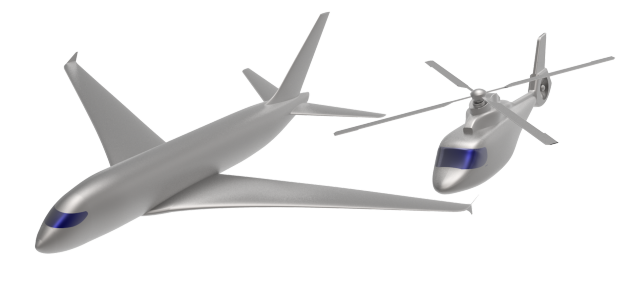
\includegraphics[scale=0.5]{1.png}
\HRule \\[0.4cm]
{ \huge \textsc{Synthèse dynamique aérospatiale\\ }} % Title of your document
\HRule \\[3cm]
 
\begin{minipage}{0.4\textwidth}
\begin{flushleft} \large
\emph{\textbf{Auteurs :}}\\
\textsc{De Leener} Maxime\\ [0,4cm]

\emph{\textbf{Cours :\ }}\\\textsc{\large LMECA 2830} % Major heading such as course name


\end{flushleft}
\end{minipage}
~
\begin{minipage}{0.4\textwidth}
\begin{flushright} \large
%\emph{\textbf{Coordinateur :}} \\
% \textsc{}\\ [0,5cm] % Supervisor's Name

\emph{\textbf{Professeur :}} \\
\textsc{Chatelain} Philippe\\
\textsc{Schrooyen} Pierre\\ [0,4cm]

\emph{\textbf{Année académique :\ }}\\\textsc{\large 2017-2018}\\[0.4cm] % Minor heading such as course title
%\emph{\textbf{Date de remise :\ }}\\\textsc{\large \textcolor{red}{24 Mars 2017}}\\


\end{flushright}
\end{minipage}\\[0cm]


~
\begin{minipage}{0.4\textwidth}

\end{minipage}

\vfill % Fill the rest of the page with whitespace

\end{titlepage}


%\tableofcontents
\newpage

\chapter{Dynamique aéronautique}

\section{Définir le range et donner son expression dans le cas d'un moteur à réaction ou d'un moteur à hélice. Comment maximiser l'endurance?}

\subsection{Rayon d'action}

\subsubsection{Définition} La connaissance du vol en palier horizontal stabilisé va nous permettre de calculer approximativement la distance franchissable ou encore rayon d’action de l’avion. Il existe trois définitions du rayon d’action.

\paragraph{Rayon d’action de sécurité} Distance horizontale maximum entre deux aéroports
que peut parcourir un avion de manière sécuritaire en effectuant un service
régulier et fiable. Pour calculer ce rayon d’action, il faut tenir compte d'énormément de facteurs comme 
\begin{itemize}
    \item carburant consommé au décollage,
    \item montée initiale/descente finale,
    \item règles de sécurité qui exigent de conserver à toutmoment suYsamment
de carburant pour pouvoir se détourner,
\item conditions météo défavorables (vent de face),
\item ...
\end{itemize}
Ceci rend le calcul extrêmement long et complexe. C’est pourquoi on utilise
également deux définitions simples mais nécessairement plus artificielles,
qui sont surtout utiles pour comparer deux appareils entre eux.

\paragraph{Rayon d’action SAR (still air range)} On suppose que l’avion décolle réservoir
plein, rejoint ses conditions de vol de croisière (altitude, vitesse) et poursuit
son vol jusqu’à épuisement du carburant. Le SAR est la distance franchie,
à l’exclusion du décollage.

\paragraph{Rayon d’action GSAR (gross still air range)} On considère un scénario encore plus
simple : soit l’avion initialement dans les conditions de vol de croisière, réservoirs
pleins. Le GSAR est la distance qu’il franchirait en palier jusqu’à
épuisement du carburant. Ce concept est évidemment extrêmement artificiel
mais il offre l’avantage d’être très simple à calculer et de fournir les
tendances du rayon d’action avec divers paramètres.

\subsubsection{Calcul du rayon d'action pour un avion à réaction}


Pour un avion à réaction, on définit la consommation spécifique comme
\begin{eqnarray}
c = \dfrac{\dot{m_c}}{T}=\dfrac{\text{débit de carburant}}{\text{poussée}}~~[\frac{kg/s}{N}]
\end{eqnarray}

\textbf{Note :} $c$ est aussi appelée $TSFC$ (Thrust Specific Fuel Consumption) dans le cours.

\begin{eqnarray}
\dfrac{dW}{dt} = -gcT
\end{eqnarray}

Or, en palier, $T=W(C_D/C_L)$. Donc,
\begin{eqnarray}
\dfrac{dW}{dt} = -\dfrac{gcC_D}{C_L}W & \text{ou encore} & dt=-\dfrac{C_L}{gcC_D}\dfrac{dW}{W}
\end{eqnarray}

La distance parcourue par l'avion en $dt$ est $dx=Vdt$, d'où
\begin{eqnarray}
dx = -\dfrac{V}{gc}\dfrac{C_L}{C_D}\dfrac{dW}{W} = -\dfrac{C_L}{C_D}\dfrac{V}{c W}dm
\end{eqnarray}
pour un avion à réaction.

\paragraph{Specific air range (SAR)}: distance parcourue en brûlant une unité de masse de carburant 
\begin{eqnarray}
SAR = \dfrac{C_L V}{cC_DW}~~[\frac{m}{kg}]
\end{eqnarray}

\paragraph{Le rayon spécifique unitaire (USAR)}: distance parcourue en brûlant une unité de masse de carburant par unité de masse de l’avion
\begin{eqnarray}
USAR = \dfrac{C_L V}{gcC_D}~~[m]
\end{eqnarray}

We can integrate this with assumptions :
\begin{eqnarray}
V=\sqrt{\dfrac{2W}{\rho C_L S}} 
\end{eqnarray}

donc soit :
\begin{itemize}
    \item $C_L,~V$ = constantes
    \item $C_L,~\rho$ (altitude) = constantes
    \item $V,~\rho$ = constantes
\end{itemize}


On obtient la formule de Bréguet-Leduc (Gross Specific Air Range for jets)
\begin{eqnarray}
GSAR &= \dfrac{C_L}{C_D}\dfrac{V}{c g} ln(\dfrac{W_1}{W_2})\\
GSAR &= USAR ln(\dfrac{W_1}{W_2})
\end{eqnarray}

Avec $W_1$ le poids initial de l'avion et $W_2$ le poids après épuisement du carburant

\subsubsection{Calcul du rayon d'action pour un avion à hélice}

Pour un avion à hélice, on utilise la notion d’efficacité du moteur plutôt que la notion de consommation spécifique, à savoir
\begin{eqnarray}
\eta_m = \dfrac{P_m}{q_c L}=\dfrac{\text{Puissance}~[W]}{\text{débit de carburant}~[kg/s]~~\text{pouvoir calorifique}~~[J/kg]}
\end{eqnarray}
car $\eta_m$ dépend peu de la vitesse, On peut alors écrire
\begin{eqnarray}
g q_c = -\dfrac{dW}{dt}=g\dfrac{W_m}{\eta_m L}
\end{eqnarray}

Le rendement de propulsion $\eta_p$ étant lui défini comme le rapport entre la puissance propulsive $w=TV$ et la puissance mécanique à l'arbre du moteur $W_m$, on en déduit
\begin{eqnarray}
\dfrac{dW}{dt}=-g\dfrac{TV}{\eta_p\eta_m L}=-\dfrac{gP}{\eta L}\dfrac{C_D}{C_L}V
\end{eqnarray}

et donc
\begin{eqnarray}
dx=-\dfrac{\eta L}{g}\dfrac{C_L}{C_D}\dfrac{dW}{W} = -\dfrac{\eta}{gSFC}\dfrac{C_L}{C_D}\dfrac{dW}{W} \\
USAR = \dfrac{\eta L}{g}\dfrac{C_L}{C_D}
\end{eqnarray}

En intégrant :

\begin{eqnarray}
R= \dfrac{\eta_p}{SFC}\dfrac{C_L}{C_D g}ln(\dfrac{W_1}{W_2})=USAR ln(\dfrac{W_1}{W_2})
\end{eqnarray}

\textbf{Note :}
avec SFC (specific fuel consumption) : $SFC=\frac{q_c}{P}=\frac{\text{fuel consumption}}{power}$
\begin{eqnarray}
P_A &= &\eta P\\
P &= &\dfrac{TV}{\eta_T}\\
\dfrac{T}{W} &= &\dfrac{D}{L}\\
\dfrac{dW}{dt} &= &-SFC g P\\
\dfrac{dW}{dt} &= &-g SFC \dfrac{W C_D V}{\eta_p C_L}
\end{eqnarray}

\subsubsection{Optimisation du rayon d'action}

\paragraph{Avion à réaction} Il faut maximiser le rapport $VC_L/C_D$. Or, parmis les trois variables $\rho,~V,~C_L$, deux sont indépendantes. Le problème d'optimisation dépendra donc de la contrainte (relation entre les variables indépendantes) imposée.
\begin{enumerate}
    \item Optimisation à $\rho$ imposé\\
    \begin{eqnarray}
    \dfrac{d}{dC_L}\left(\dfrac{V C_L}{C_D}\right)_\rho=0
    \end{eqnarray}
    On sait que
    \begin{eqnarray}
    \dfrac{VC_L}{C_D}\propto \dfrac{C_L^{1/2}}{C_D}
    \end{eqnarray}
    Avec la polaire parabolique, on obtient alors un optimum pour
    \begin{eqnarray}
    \left. C_L\right|_{rao}=\sqrt{\dfrac{C_{D,0}}{3k}}&\rightarrow & V_{rao}=\sqrt{\dfrac{2W}{\rho S}}\left(\dfrac{3k}{C_{D,0}}\right)^{1/4}
    \end{eqnarray}
    
    \item Optimisation à position de la manette des gaz imposée\\
    Cela impose :
    \begin{eqnarray}
    T(\rho,\Pi)=\rho\dfrac{V^2}{2}SC_D
    \end{eqnarray}
    avec $\Pi$ la position de la manette des gaz. A $\Pi$ donnée, on suppose la poussée $T$ proportionnelle à $\rho$ :
    \begin{eqnarray}
    T_0(\Pi)=\rho_0\dfrac{V^2}{2}SC_D~~\rightarrow~~V\propto C_D^{-1/2}~~\rightarrow~~\dfrac{VC_L}{C_D}\propto\dfrac{C_L}{C_D^{3/2}}
    \end{eqnarray}
    Avec la polaire parabolique, on obtient alors un optimum pour
    \begin{eqnarray}
    \left. C_L\right|_{rao}=\sqrt{\dfrac{C_{D,0}}{2k}}&\rightarrow & V_{rao}=\sqrt{\dfrac{2W}{\rho S}}\left(\dfrac{2k}{C_{D,0}}\right)^{1/4}
    \end{eqnarray}
    L'altitude correspondante à l'optimum résulte alors de l'équation de sustentation
    \begin{eqnarray}
    \rho = \dfrac{2W}{V^2SC_L}
    \end{eqnarray}
    
    \item Optimisation à V imposée\\
    Dans ce cas, la solution est élémentaire, l’optimum est atteint pour l’incidence de finesse maximum. Dans ce cas également, $\rho$ est déduit de l’équilibre en sustentation.
\end{enumerate}

\textbf{Note :} Parmis les 3 optimisation, c'est certainement la première qui a le plus de signification pratique.\\
\begin{eqnarray}
GSAR_{opt} = \dfrac{C_L V_{rao}}{gcC_D}ln\dfrac{W_1}{W_2}
\end{eqnarray}

Etant donné que $V_{rao}\propto\sqrt{\frac{P}{S}}$, il apparaît que le rayon d'action est fonction croissante de la charge alaire $P/S$ (que l'on augmente en réduisant la surface alaire et non en augmentant le poids!). L'augmentation du rayon d'action est donc en contradiction avec la réduction de la vitesse d'atterrissage/décollage. Enfin, comme $V_{rao}\propto(\frac{k}{C_{D,0}})^{1/4}$ mais que par ailleurs, $(C_L/C_D)_{rao}\propto (kC_{D,0})^{-1/2}$, on augmente le rayon d'action en réduisant k (càd en aumentant l'allongement) mais surtout $C_{D,0}$.

\paragraph{Avion à hélice} Dans le cas de l’avion à hélice, la vitesse n’intervenant pas dans l’expression du USAR, le rayon d’action maximum s’obtient en maximisant la finesse $C_L/C_D$, quelle que soit la contrainte imposée (altitude, position de la manette des gaz ou vitesse).

\subsection{Endurance}


L’endurance est le temps de vol correspondant au rayon d’action GSAR. 

\subsubsection{Avion à réaction}
\begin{eqnarray}
\dfrac{dP}{dt}=-gcE=-g\cdot TSFC\cdot E\\
E=\dfrac{C_L}{g\cdot TSFC\cdot C_D}ln(\dfrac{W_1}{W_2})
\end{eqnarray}
et l’on voit que l’endurance est optimisée à l’incidence de finesse maximum.

\subsubsection{Avion à hélice}

\begin{eqnarray}
\dfrac{dP}{dt}=-\dfrac{gP}{\eta L}\dfrac{C_D}{C_L}V~~\rightarrow~~dt=-\dfrac{\eta L}{g}\dfrac{C_L}{VC_D}\dfrac{dP}{P}\\
E=\dfrac{\eta_p}{gSFC}\dfrac{C_L^{3/2}}{C_D}\sqrt{2\rho S}(W_1^{-1/2}-W_0^{-1/2})
\end{eqnarray}

L'endurance est donc optimisée en maximisant $\dfrac{\eta L}{g}\dfrac{C_L}{VC_D}$


\section{Définir la stabilité statique, dynamique et le contrôle d'un avion.}


\paragraph{Stabilité statique} étude de la tendance initiale d'un véhicule à retourner à son point d'équilibre après perturbation.

\paragraph{Stabilité dynamique} étude de l'historique temporel de la réponse à une perturbation.

\paragraph{Contrôle} étude du changement d'une configuration à une autre de l'avion.



\section{Définir la marge statique. Comment cela dépend-il de $C_{L\alpha}$ ? Est-ce qu'un grand $C_{L\alpha}$ est bon pour la stabilité ?}

La \textbf{marge statique} est la distance entre le \textbf{centre de gravité} et le \textbf{point neutre}.

Le \textbf{point neutre} est le point pour lequel la raideur en tangage s’annule. Il définit la frontière entre centrages stables et instables.

Sachant que la raideur en tangage s'exprime comme 
\begin{eqnarray}
C_{m\alpha}=C_{L\alpha}(h-h_n)
\end{eqnarray}

la marge statique peut être définie comme
\begin{eqnarray}
h_n-h=-\dfrac{C_{m\alpha}}{C_{L\alpha}}
\end{eqnarray}

Puisque $C_{m\alpha}$ doit être négatif pour que l'avion soit statiquement stable, $h_n-h$ doit donc être positif, c'est-à-dire que le centre de gravité doit se trouver en avant du point neutre. (Ordre de grandeur : marge statique constamment plus grande ou égale à 5$\%$ de la corde aérodynamique moyenne. Donc si $C_{L\alpha}$ devient trop grand, la marge statique passera sous cette valeur et l'appareil ne sera pas assez stable.


 

\section{Vol plané en descente sans moteur : donnez les forces en jeu, distance franchissable,...}

Premièrement, il n'y a pas de poussée : $T=0$ et donc $L<W$ (la portance $<$ le poids de l'appareil).

\begin{figure}[h!]
    \centering
    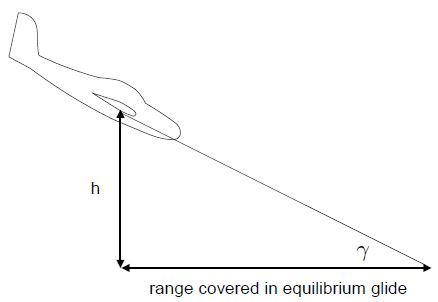
\includegraphics[scale=0.6]{12.JPG}
    \caption{Avion en train de planer}
    \label{12}
\end{figure}

Soit $\gamma$ la pente de descente de l'avion.

\textbf{L'équation d'équilibre} de l'avion en vol plané devient :
\begin{eqnarray}
L &= &Wcos(\gamma)\\
-D &= &W sin(\gamma)
\end{eqnarray}
avec \begin{itemize}
    \item $D$ : la force de traînée
    \item $W$ : le poids de l'appareil
    \item $L$ : la portance
\end{itemize}

La vitesse est donc maintenue uniquement par $W sin(\gamma)$.

Dans ce cas, la pente de descente vaut :
\begin{eqnarray}
tan(\gamma) = -\dfrac{D}{L} = -\dfrac{C_D}{C_L} = \dfrac{1}{f}
\end{eqnarray}

avec $f=\dfrac{C_L}{C_D}$ la \textbf{finesse}.

La \textbf{distance maximum franchissable} est donc obtenue en minimisant $|tan(\gamma)|$, donc en planant à \textbf{finesse maximum} et donc \textbf{indépendamment du poids} de l'avion.

\begin{eqnarray}
tan(\gamma) = -\dfrac{D}{L}=-\dfrac{C_D}{C_L}\\
Range_{gliding}=\int_H^0\dfrac{dH}{tan(\gamma)}
\end{eqnarray}

On peut également calculer la vitesse de descente $w_d$ :

\begin{eqnarray}
w_d=\dfrac{R}{D}=\sqrt{\dfrac{2W}{\rho S}}cos^{\frac{3}{2}}(\gamma)\dfrac{C_D}{C_L^{\frac{3}{2}}}
\end{eqnarray}

\begin{eqnarray}
L &= &\dfrac{1}{2}\rho V^2 S C_L\\
D &= &\dfrac{1}{2}\rho V^2 S C_D
\end{eqnarray}


\section{Expliquer pourquoi un avion a tendance à voler à ailes horizontales ? Comment peut-on accroître cet effet ?}

En considérant \textbf{un seul degré} de liberté de roulis, il n'y a pas de raideur du premier ordre qui pousserait l'avion à voler à l'horizontal.

Or, lorsqu'on lève cette hypothèse, il apparaît (lorsque l'avion roule de $\Phi$) une \textbf{composante de gravité} $mgsin(\Phi)$ dans la direction y, d'où une composante de dérapage et $\beta>0$ et donc un \textbf{couple redresseur} $C_{l\beta}$ (ainsi qu'un couple $C_{n\beta}\beta$ créant le virage : effet girouette).

L'effet dièdre par la dérivée $C_{l\beta}$ permet d'expliquer cette tendance des avions à voler à ailes horizontales.

Plusieurs facteurs contribuent à cela, les plus importants provenants de la \textbf{géométrie des ailes} :
\begin{enumerate}
    \item \textbf{Effet de l'angle de dièdre $\Gamma$ des ailes}\footnote{http://asaero.chez.com/Conseils/diedre2.htm}\\
    
    \begin{figure}[h!]
    \centering
    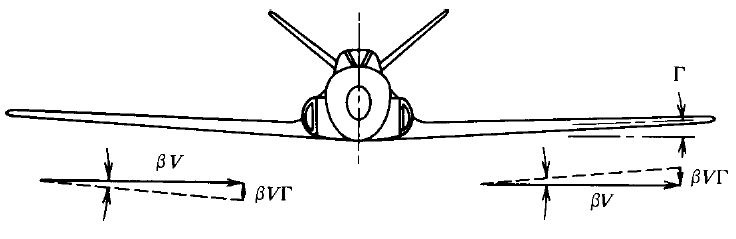
\includegraphics[scale=0.6]{32.JPG}
    \caption{Rôle du dièdre}
    \label{32}
    \end{figure}
    
    La vitesse normale \begin{itemize}
        \item  sur l'aile de droite : $V_n=wcos(\Gamma) + vsin(\Gamma) = w+v\Gamma$
        \item sur l'aile de gauche : $V_n = w-v\Gamma$
    \end{itemize}
    La variation de $\Delta\alpha$ de l'angle d'attaque due au dièdre est donc :$\Delta\alpha=v\Gamma/V= sin(\beta)\Gamma\approx \pm\beta\Gamma$.\\
    L'aile côté vent a un angle d'attaque accru (portance accrue) et vice-versa.\\
    Donc, le bilan est un \textbf{couple de roulis} $L<0$ si $\Gamma>0$, prtaiquement linéaire en $\beta$ et $\Gamma$ soit un $C_{l\beta}<0$ fixé pour un $\Gamma>0$
    
    
    \item \textbf{Effet de fuselage}\\
    
    \begin{figure}[h!]
    \centering
    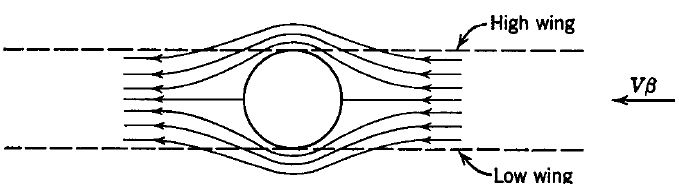
\includegraphics[scale=0.6]{34.JPG}
    \caption{Effet du fuselage sur $C_{l_\beta}$}
    \label{34}
    \end{figure}
    
    On voit (figure \ref{34}) que l'écoulement autour du fuselage induit par le dérapage a tendance à augmenter/réduire l'incidence sur l'aile tribord selon que l'aile soit en position haute ou basse et réciproquement pour l'aile bâbord. On en conclu que l'interférence aile et fuselage produit une contribution négative à $C_{l_\beta}$ pour une aile haute (effet dièdre \textbf{accru}) et positive pour une aile basse (effet dièdre \textbf{aténué}). C'est la raison pour laquelle les ailes hautes ont un dièdre moins important que les ailes basse, surtout pour les ailes en flèches, pour lesquelles on peut même observer parfois des dièdres négatifs. 
    
    La grandeur de l'effet dépend dans les deux cas de la \textbf{longueur du fuselage en amont de l'aile et de sa forme}.
    
    \item \textbf{Effet de la flèche}\\
    
    \begin{figure}[h!]
    \centering
    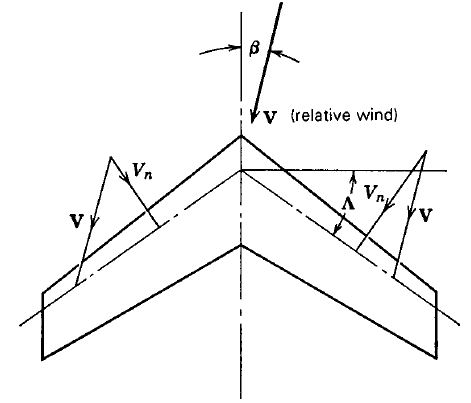
\includegraphics[scale=0.6]{33.JPG}
    \caption{Effet de la flèche sur $C_{l_\beta}$}
    \label{33}
\end{figure}
    
    La portance est déterminée par la composante de $V$ perpendiculaire au bord d'attaque de l'aile. Celle-ci sera \textbf{plus importante du côté du vent relatif} que de l'autre côté, donc $C_{l\beta}<0$. La flèche a donc le même effet que le dièdre. Elle augmente même l'effet dièdre (5 degrés de flèches arrière valent 1 degré de dièdre. 

\item \textbf{Effet de la dérive}\\

Enfin, la dernière contribution importante à $C_{l_\beta}$ est celle de la dérive. La portance sur la dérive résultant d'un dérapage produit en effet un couple de roulis égal à $L_Fz_F$, où $z_F$ est la distance entre le centre aérodynamique de la dérive et l'axe $x$. Par conséquent, le coefficient de couple de roulis vaut
\begin{eqnarray}
\Delta C_l=a_F(-\beta+\sigma)\dfrac{z_FS_F}{Sb}\left(\dfrac{V_F}{V}\right)^2
\end{eqnarray}

et la contribution à $C_{l_\beta}$
\begin{eqnarray}
\Delta C_{l_\beta}=-a_F\left(1-\dfrac{\partial\sigma}{\partial \beta}\right)\dfrac{z_FS_F}{Sb}\left(\dfrac{V_F}{V}\right)^2
\end{eqnarray}

\begin{figure}[h!]
    \centering
    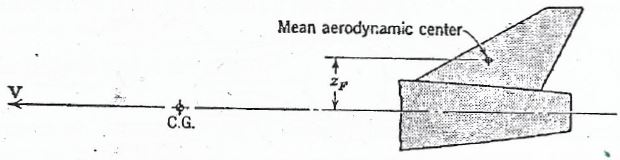
\includegraphics[scale=0.6]{35.JPG}
    \caption{Schéma de la dérive}
    \label{35}
\end{figure}
\end{enumerate}

Le guidage en roulis est effectué grâce aux ailerons qui sont le plus souvent des volets mobiles de l'aile principale braqués de manière différentielle comme indiqué sur la figure \ref{36}.

\begin{figure}[h!]
    \centering
    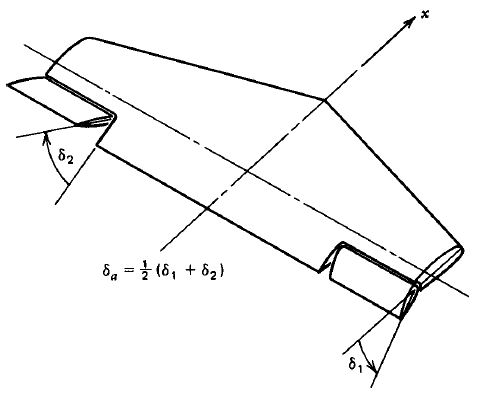
\includegraphics[scale=0.6]{36.JPG}
    \caption{Schéma de la dérive}
    \label{36}
\end{figure}

\section{Lacet inverse et lacet induit : expliquez, comment les éviter ?}

La manoeuvre de virage est commandée par les ailerons en créant un couple de roulis. Cette commande entraîne des \textbf{effets secondaire : le lacet inverse}.

\textbf{L'efficacité des ailerons} se mesure par : $dC_l/d\delta_a$ et $dC_n/d\delta_a$ avec $\delta_a = (\delta_1+\delta_2)/2$.

Pour $\delta_i >0$ (aileron droit \textbf{descend}), on vire à gauche. L'accroissement de la portance à droite et la diminution à gauche, ainsi que le mouvement de virage (vitesse plus importante de l'aile de droite que l'aile de gauche) conduisent à une \textbf{traînée plus importante sur l'aile droite} que sur l'aile gauche. Et cela produit donc un lacet \textbf{positif}.

Cet effet contrecarre l'effet souhaité :
\begin{itemize}
    \item \textbf{lacet induit} dû à la différence de vitesse des ailes 
    \item \textbf{lacet inverse} dû à la différence de traînée 
\end{itemize}

Pour contrer ces effets :

\begin{itemize}
    \item \textbf{ailerons Frise} : d'un côté l'aileron descend et de l'autre l'aileron monte (augmentation de la traînée de chaque côté)
    \item \textbf{braquage différentiel} : l'angle de l'aileron montant est plus important que celui descendant afin d'égaliser les traînées.
    \item \textbf{utilisation d'aérofreins (spoilers)} : augmentent la traînée du côté bas, lent (intérieur au virage)
    \item Actionnement du palonnier afin d'engendrer un effet de la dérive.
\end{itemize}

\subsubsection{Réponses impulsionnelles pour un échelon de $\Delta\delta_e=1\degree$}

À partir des fonctions de transfert, on calcule aisément la réponse à un échelon d’angle de gouverne. On a représenté aux figures \ref{61}–\ref{62} les évolutions de la vitesse, de l’incidence et de la pente de la trajectoire consécutives à un échelon d’un degré d’angle de gouverne. 

On observe à la figure \ref{61} qui montre les 10 premières secondes de la réponse,
que seul l’angle d’incidence répond rapidement au déplacement de la gouverne, et que son évolution est dominée par le mode bien amorti d’oscillation d’incidence. Au contraire, les variables de trajectoire (vitesse et pente) répondent beaucoup plus lentement. On observe à la figure \ref{62} qui présente l’évolution des variables sur une durée de 10 minutes, que les transitoires persistent très longtemps, et qu’après quelques secondes, c’est le mode phugoïde qui domine
l’évolution.

L’état de régime approché si lentement se caractérise par une vitesse plus élevée, correspondant à la diminution d’incidence attendue comme suite au braquage vers le bas de la gouverne. La pente de la trajectoire change à peine (augmentation d’environ $0,1\degree$). L’augmentation s’explique par le fait que le vol de départ est à une vitesse inférieure à la vitesse de traînée minimale.

Si l’objectif du braquage de la gouverne était de modifier les conditions de vol, on ne peut pas dire que la manoeuvre soit une réussite. Manifestement, un guidage longitudinal satisfaisant exige une manoeuvre un peu plus sophistiquée, qu’elle soit effectuée par un pilote humain ou automatique.

\begin{figure}[h!]
    \centering
    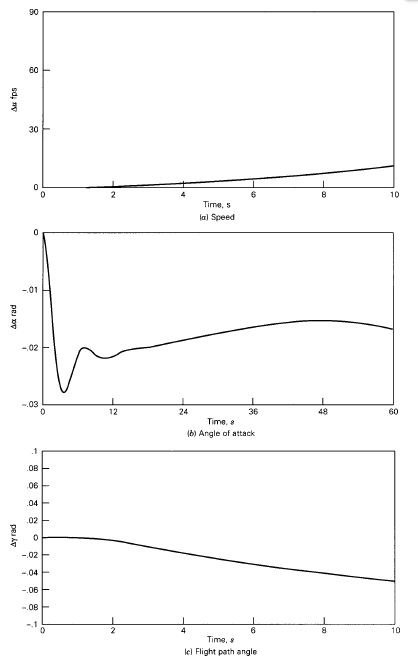
\includegraphics[scale=0.6]{61.JPG}
    \caption{Réponse à un échelon d’angle de gouverne ($\Delta\delta_e=1\degree$)}
    \label{61}
\end{figure}

\begin{figure}[h!]
    \centering
    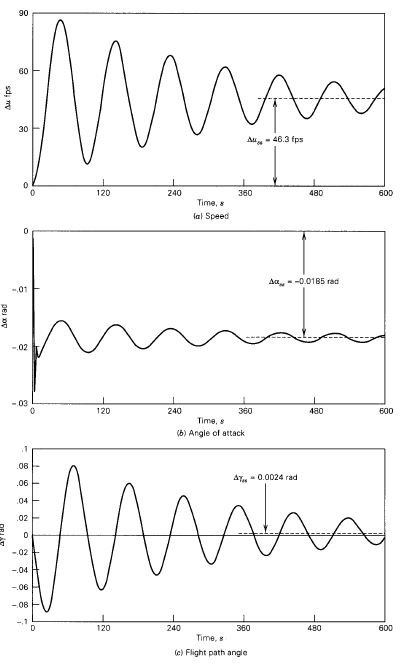
\includegraphics[scale=0.6]{62.JPG}
    \caption{Réponse à un échelon d’angle de gouverne ($\Delta\delta_e=1\degree$)}
    \label{62}
\end{figure}


%%%%%%%%%%%%%%%%%%%%%%%%%%%%%%%%%%%%%%%%%%%%%%%%%%%%%%%%%%%%%%%%%%%%%%%%%%%%%%%%%%%%%%%%%%%%%%%%%%%%%%%%%%%%%%%%%%%%%%%%%%%


\chapter{Dynamique spatiale}

\section{Citez les types de moteurs de fusée}

\begin{itemize}
    \item Moteurs à ergols solides (solid propellant)
    \item Moteurs à ergols liquides (liquid propellant)
\end{itemize}

Dans ces deux cas, ce sont des moteurs à propulsion chimique. L'avantage de tels modes est qu'ils ne font aucuns prélèvement au milieu et donc peuvent être utilisés dans le vide (l'espace). La propulsion chimique est une propulsion au cours de laquelle la poussée est fournie pas le produit d'une réaction chimique, la plupart du temps par combustion (ou oxydation) d'un carburant. Une réaction chimique combine deux ou plus de sortes de produits chimiques et produit différents produits chimiques. Une réaction couramment utilisée est une réaction qui combine du di-hydrogène et du di-oxygène pour faire de l'eau. Généralement, la réaction produit aussi de la chaleur qui va chauffer le produit. Lorsqu'un produit est chauffé, il se dilate et va être éjecté de la tuyère avec une certaine énergie cinétique. C'est ce qui produit la poussée.

La réaction chimique qui se produit dans la chambre de combustion est par exemple:
\begin{eqnarray}
O_2+2H_2~\rightarrow~2H_2O
\end{eqnarray}

\section{Expliquez le principe des moteurs de fusée à carburant solide}

Dans ce type de moteur, le combustible et le comburant sont mélangés ensemble dans dans un ergols\footnote{Un ergol, dans le domaine de l'astronautique, est une substance homogène employée seule ou en association avec d'autres substances et destinée à fournir de l'énergie. Les ergols sont les produits initiaux, séparés, utilisés dans un système propulsif à réaction. Ils sont constitués d'éléments oxydants (comburant) et réducteurs (carburant ou combustible). Les termes correspondants en anglais sont propellant et fuel.} solides. Le tout est empaqueté sous forme de cylindre. La chambre de combustion est simplement un trou au centre du cylindre et la combustion prend place à la surface des ergols solides. Cette combustion produit une grande quantité de gaz d'échappements à haute pression et température. Le gaz d'échappement passent ensuite à travers une tuyère (nozzle) qui accélère le flux. La poussée est alors produite par conservation d'énergie et principe d'action/réaction. 

La quantité de poussée produite par la fusée dépend du design de la tuyère. La plus petite aire transversale de la tuyère est appelée \textit{col} (throat). Les gaz chauds d'échappement sont "\textit{choked}" (nombre de Mach = 1) au col, c'est à dire qu'en amont du col, la vitesse du gaz est subsonique et en aval supersonique. Cela signifie que le débit massique $\dot{m}$ est déterminé par l'aire du col. Le ratio d'aire entre le col et l'aire de sortie $A_e$ fixe la vitesse de sortie $V_e$ et la pression de sortie $p_e$. 

La pression de sortie n'est égale à la pression extérieure que dans certaines conditions. Nous devons, par conséquent, utiliser la longue version de l'équation de poussée générale pour décrire la poussée du système. Si la pression extérieure est donnée par $p_0$, l'équation de la poussée $T$ devient :

\begin{eqnarray}
T &= &\oint_{internal}pdS+P_\infty (A_i-A_e)\\
(\dot{m}_{air}+\dot{m}_{fuel})u_e-\dot{m}_{air}u_i &= &\oint_{internal}pdS+P_\infty (A_i-A_e)\\
 & \Downarrow &\text{Pour un moteur de fusée}\\
T &= &\dot{m}\cdot u_e +(p_e-p_\infty)\cdot A_e
\end{eqnarray}

Notons que le comburant est mélangé au combustible, les fusées solides peuvent donc générer de la poussée dans le vide (espace), où il n'y a pas de source d'oxygène. 

\begin{figure}[h!]
    \centering
    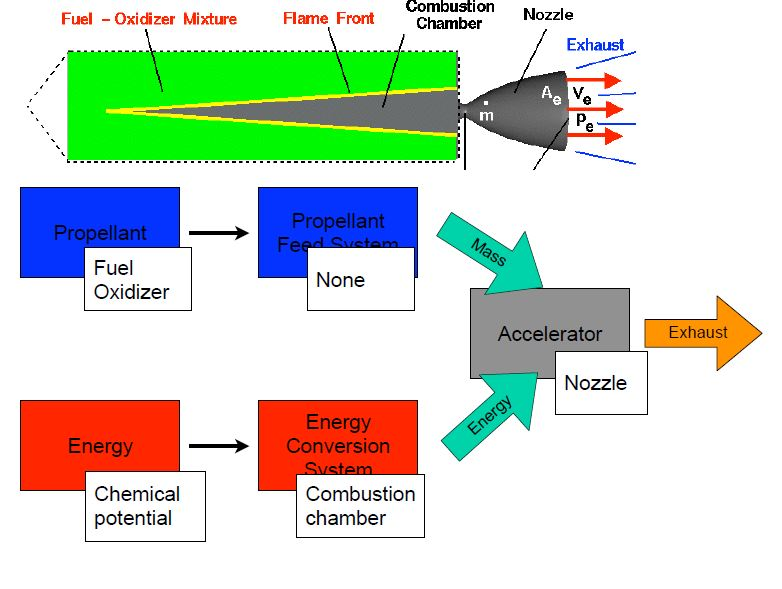
\includegraphics[scale=0.6]{40.JPG}
    \caption{Moteur de fusée à ergol solide}
    \label{40}
\end{figure}



\section{Expliquez le principe des moteurs de fusée à carburant liquide}

Dans une fusée à ergols liquides, le combustible et le comburant stockés sont pompés dans une chambre de combustion où ils sont mélangés et brûlé. Cette combustion produit une quantité importante de gaz d'échappement à haute température et pression.

Notons que la suite du moteur à ergols liquides est exactement le même que celui à ergols solides.

\begin{figure}[h!]
    \centering
    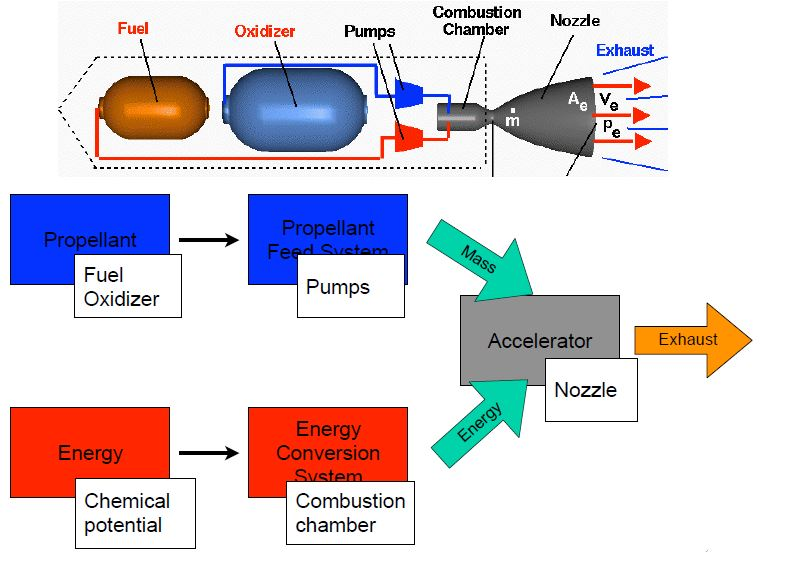
\includegraphics[scale=0.6]{41.JPG}
    \caption{Moteur de fusée à ergol liquide}
    \label{41}
\end{figure}



\section{Expliquer le problème pouvant survenir au niveau de la tuyère, et des solutions pour y remédier}

Pour qu'une tuyère d'un moteur-fusée contribue de manière optimale à l'accélération des gaz (tuyère adaptée), il est nécessaire qu'elle soit relativement longue. Dans le cas de la fusée Ariane 5 par exemple, la tuyère du moteur Vulcain devrait, pour produire la poussée optimale, avoir une longueur de 7 mètres. Les divergents des moteurs propulsant les étages supérieurs des lanceurs doivent être particulièrement longues car la pression externe est quasi nulle. La longueur de la tuyère entraîne un allongement du lanceur et donc un alourdissement de la structure ce qui est préjudiciable aux performances globales.

\begin{itemize}
    \item Une tuyère de moteur-fusée propulsant de premier étage est amenée à fonctionner dans des conditions de pression externe très différentes : celle-ci est de 1 bar au lancement mais quasi nulle lorsque le moteur s'éteint. La géométrie de la tuyère ne peut s'adapter aux variations continues de la pression externe. Le choix effectué est sous détendre les gaz en sortie du divergent c'est-à-dire que sa pression est supérieure à celle de l'air ambiant sur la majorité du temps de fonctionnement de l'étage. Ceci permet de disposer d'une tuyère courte dont à raccourcir la masse du lanceur.
    \item Toutefois au moment de la montée en puissance du moteur-fusée avant le décollage et à l'extinction du moteur les gaz produits sont temporairement en sur-détente ce qui crée un décollement des flux pouvant endommager la tuyère au décollage et générer des poussées non symétriques au décollage comme à l'extinction.
\end{itemize}

\begin{figure}[h!]
    \centering
    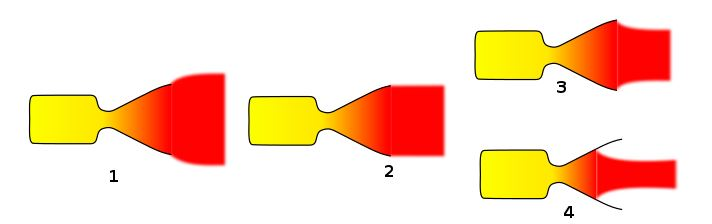
\includegraphics[scale=0.6]{44.JPG}
    \caption{Régimes de fonctionnement d'une tuyère de moteur-fusée en fonction de l'écart entre la pression des gaz en sortie du divergent et la pression extérieure ambiante. De gauche à droite :\\
1. Sous-détente des gaz en sortie de divergent : la pression ambiante est inférieure à la pression des gaz\\
2. Tuyère adaptée : égalité de la pression des gaz en sortie et de la pression ambiante (régime optimal)\\
3. Sur-détente des gaz en sortie du divergent\\
4. Sur-détente importante des gaz en sortie du divergent avec décollement du flux le long de la paroi du divergent}
    \label{44}
\end{figure}

\begin{figure}[h!]
\centering
\begin{minipage}{.5\textwidth}
  \centering
    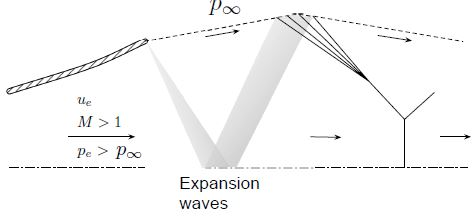
\includegraphics[scale=0.6]{45.JPG}
    \caption{Tuyère sous-détendue}
    \label{45}
\end{minipage}%
\begin{minipage}{.5\textwidth}
  \centering
    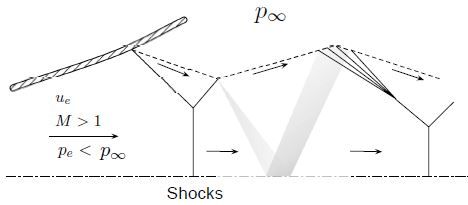
\includegraphics[scale=0.6]{46.JPG}
    \caption{Tuyère sur-détendue}
    \label{46}
\end{minipage}
\end{figure}

\subsection{La forme de la tuyère devrait être adaptée avec l'altitude}

Il y a deux types de tuyère :
\begin{itemize}
    \item Délimitée : l'expansion est imposée par la géométrie de la tuyère
    \item Libre d'expansion : l'expansion répond à la pression ambiante
\end{itemize}

\begin{figure}[h!]
    \centering
    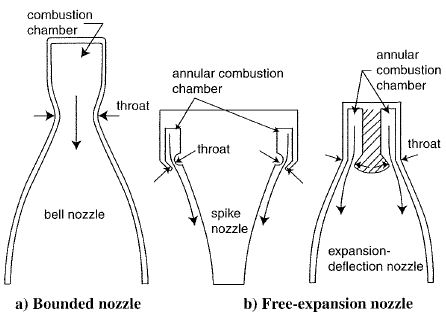
\includegraphics[scale=0.6]{47.JPG}
    \caption{Différents types de tuyères}
    \label{47}
\end{figure}

La forme du divergent doit être telle que sa paroi se confond avec la ligne de courant de l'écoulement des gaz expulsés. Ce profil se calcule généralement en résolvant les équations d'Euler en particulier en utilisant la méthode des caractéristiques. Le profil optimal est celui d'un cône dont le demi-angle au sommet est de 15°. Afin de raccourcir la longueur du divergent et ainsi de réduire la longueur du lanceur et donc sa masse deux solutions sont mises en œuvre :

\begin{itemize}
    \item \textit{La tuyère idéale tronquée} (TIC) est une tuyère dont le profil suit la courbe optimale mais qui est amputée de son extrémité. Dans le cas du moteur Vulcain, le fait de tronquer de 2/3 le profil idéal (longueur de 2,5 mètres au lieu de 7 mètres) entraîne une perte de poussée limitée à 3 $\%$.
    \item \textit{La tuyère optimisée à choc interne} (TOC = Thrust-Optimized Contour) est une tuyère dont le profil s'écarte de la courbe optimale ce qui permet de gagner encore 20 $\%$ sur la longueur du divergent par rapport à une tuyère de type TIC. L'angle au voisinage du col (de 20 à 50°) est supérieur à l'angle optimal ce qui permet d'accroître plus rapidement le diamètre du divergent. L'écart par rapport au profil idéal se réduit progressivement pour ne plus atteindre qu'environ 10$\degree$ à l'extrémité du divergent. La forme obtenue est dite en coquetier. Ce gain s'obtient au prix d'un écoulement du gaz plus perturbé qui peut donner lieu à des ondes de choc interne dans le divergent.
\end{itemize}

\begin{figure}[h!]
    \centering
    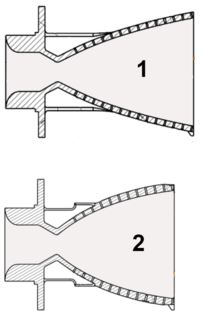
\includegraphics[scale=0.6]{48.JPG}
    \caption{Comparaison des sections de tuyère de moteur-fusée de type : 1 - TIC : Tuyère idéale tronquée 2 - TOC Tuyère en coquetier}
    \label{48}
\end{figure}

Une autre manière de réduire la longueur du divergent est de multiplier le nombre de tuyères associés à une unique chambre de combustion. Le débit de chaque tuyère étant le quart du débit total, la taille du col est réduite et en conséquence le diamètre et la longueur du divergent.

\subsubsection{Tuyère à divergent extensible}

Les moteurs-fusées d'étage supérieur nécessitent des tuyères très longues car elles fonctionnent dans le vide. Pour limiter la masse structurelle qu'imposerait une tuyère très longue certains moteurs comme le RL-10 B-2 qui propulse le second étage du lanceur Delta IV, comportent un divergent extensible qui n'est complètement déployé que lorsque l'étage inférieur a été largué.

\begin{figure}[h!]
    \centering
    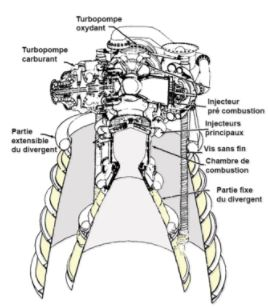
\includegraphics[scale=0.8]{49.JPG}
    \caption{Schéma du RL-10 à divergent extensible.}
    \label{49}
\end{figure}

\subsubsection{Tuyère à écoulement externe/corps central (par ex aerospike)}

La tuyère aerospike est un type de tuyère expérimenté sur les moteurs-fusées à ergols liquides qui permet d'optimiser l'efficacité de la propulsion dans une large gamme d'altitudes ( = de pression atmosphérique). Un moteur-fusée équipé d'une tuyère aerospike utilise 25 à 30 $\%$ de carburant en moins à basse altitude là où les lanceurs ont besoin des poussées les plus importantes. Ce type de tuyère fait l'objet d'études depuis le début de l'ère spatiale mais sa mise au point se heurte au problème de refroidissement de la rampe qui canalise le jet de gaz. Seuls des prototypes de ce type de tuyère ont été construits. La tuyère aerospike joue notamment un rôle central dans l’architecture des projets de lanceurs orbitaux monoétages (SSTO) dont les moteurs doivent fonctionner dans une gamme de pression allant de la pression au niveau de la mer jusqu'au vide.

\begin{figure}[h!]
    \centering
    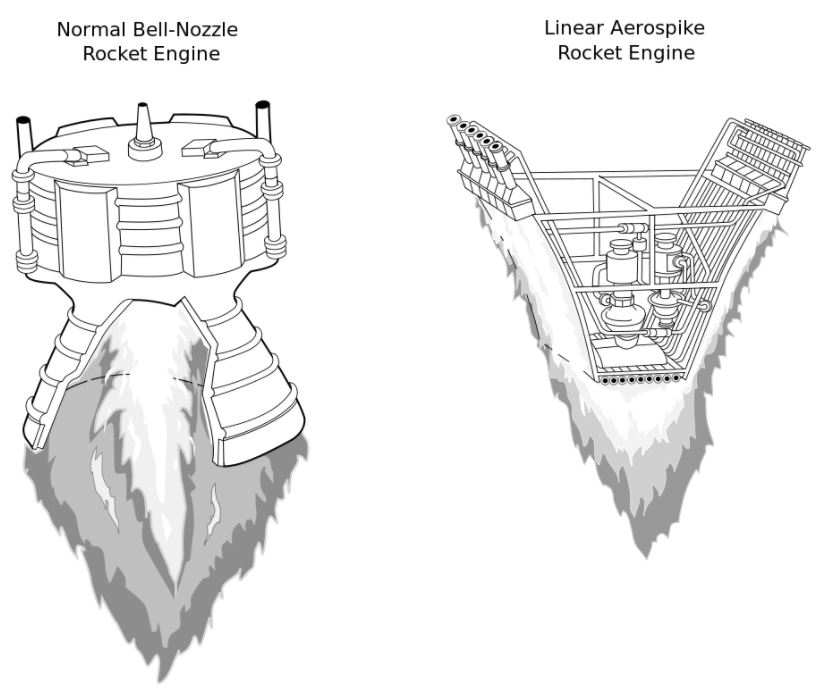
\includegraphics[scale=0.4]{50.JPG}
    \caption{Schéma comparant deux moteurs-fusées mettant en œuvre d'une part une tuyère classique et d'autre part une tuyère de type Aerospike.}
    \label{50}
\end{figure}

\paragraph{Principe de la tuyère aérospike}

Les moteurs-fusées classiques ne donnent le meilleur de leur performance qu'à une altitude donnée. Le rendement du moteur-fusée est en effet déterminé par la forme de la tuyère qui est fixe. Dans celle-ci les gaz brûles se détendent et transforment leur énergie thermique en énergie cinétique à l'origine de la poussée qui propulse la fusée. La forme et la longueur de la tuyère déterminent la pression de sortie des gaz brûlés ; or pour que le moteur fonctionne à son meilleur rendement, il est nécessaire que cette pression de sortie soit égale à la pression atmosphérique externe. Pour optimiser la poussée du moteur il serait nécessaire que la pression des gaz en sortie diminue progressivement (allongement de la tuyère et évolution de sa forme) au fur et à mesure que la fusée s'élève et que la pression atmosphérique ambiante diminue.

La tuyère de type aerospike apporte une solution au problème de l'adaptation de la tuyère à la pression ambiante. Avec ce type de tuyère les gaz en sortie de la chambre de combustion sont éjectés, non pas dans une tuyère aux parois fixes mais le long d'une structure fixe (la rampe). Les gaz se détendent en étant canalisés d'une part par la rampe d'autre part par la masse d'air ambiante. Par cette méthode la pression des gaz éjectés s'adapte automatiquement à la pression ambiante. Différentes formes de tuyère aerospike ont été étudiées : linéaire, annulaire... La rampe peut se terminer par une pointe ou être tronquée en expulsant des gaz formant une zone de surpression la prolongeant. Les gaz peuvent être produits par plusieurs chambres de combustion placés en couronne autour de la rampe centrale ou par une chambre unique qui les expulse à travers une fente annulaire.

L'idée derrière la conception de la tuyère aerospike est qu'à basse altitude, la pression ambiante comprime le jet de gaz contre la rampe centrale. La recirculation dans la zone de base de la rampe permet d'élever la pression ambiante à proximité. Comme la pression sur le dessus du moteur est ambiante, cela signifie que la base ne donne aucune poussée générale (mais cela signifie aussi que cette partie de la tuyère ne perd pas de poussée en formant un vide partiel, donc la partie de base de la tuyère peut être ignorée à basse altitude).

Lorsque la fusée prend de l'altitude, la pression d'air qui comprime le jet de gaz contre la rampe diminue, mais la pression au-dessus du moteur diminue en même temps et ce n'est donc pas nuisible. En outre, bien que la pression de base chute, la zone de redirection maintient la pression sur la base jusqu'à une fraction de 1 bar, une pression qui n'est pas équilibrée par le vide à proximité sur le dessus du moteur; cette différence de pression donne une poussée supplémentaire en altitude, créant un effet de compensation d'altitude. Cela produit le même effet que celui d'une cloche qui devient plus grande à mesure que la pression baisse, fournissant une compensation d'altitude.

Les inconvénients des moteurs aerospike sont le poids supplémentaire de la rampe centrale mais surtout la nécessité de refroidir suffisamment la rampe directement frappée par les jets de gaz en sortie de la chambre de combustion. En outre, la plus grande surface refroidie peut réduire les performances en deçà des niveaux théoriques en réduisant la pression contre la tuyère. De plus, les moteurs aerospike ont un rendement faible lorsque la vitesse est peu élevée (Mach 1-3) car le flux d'air autour du véhicule n'exerce pas assez de pression, ce qui diminue la poussée.




\section{Définir l'impulsion spécifique et la vitesse d'échappement équivalente et donner un ordre de grandeur}

Reprenons l'équation de la poussée et divisons la par $\dot{m}$ :
\begin{eqnarray}
\dfrac{T}{\dot{m}} = u_e+(p_e-p_0)\dfrac{A_e}{\dot{m}}
\end{eqnarray}

Nous définissons une nouvelle vitesse dire \textit{vitesse équivalent} $c$ :
\begin{eqnarray}
c = u_e+(p_e-p_0)\dfrac{A_e}{\dot{m}}
\end{eqnarray}

de sorte que
\begin{eqnarray}
T = \dot{m} \cdot c
\end{eqnarray}

\textbf{L'impulsion totale ($I$)} d'une fusée est définie comme la moyenne de la poussée multipliée par le temps total du tir (firing). Définissons le temps total comme $\Delta t$ :

\begin{eqnarray}
I=T\cdot\Delta t
\end{eqnarray}

Puisque la poussée peut changer avec le temps, nous pouvons aussi définir une équation intégrale pour l'impulsion totale. 
\begin{eqnarray}
I &= &\int T dt\\
I &= &\int(\dot{m} c)dt
\end{eqnarray}

On peut donc intégrer cette équation :
\begin{eqnarray}
I = m\cdot c
\end{eqnarray}

où $m$ est la masse totale d'ergols. Nous pouvons diviser cette équation par le poids des ergols pour définir \textbf{l'impulsion spécifique}. Le mot "spécifique" signifie simplement "divisé par le poids". L'impulsion spécifique $I_{sp}$ est donnée par :
\begin{eqnarray}
I_{sp}  = \dfrac{c}{g_0}
\end{eqnarray}

avec $g_0$, l'accélération gravitationnelle au niveau de la mer. Maintenant, nous pouvons l'exprimer en fonction de la poussée :
\begin{eqnarray}
I_{sp} = \dfrac{T}{\dot{m} g_0}~~[sec]
\end{eqnarray}

Pourquoi sommes-nous intéressé par l'impulsion spécifique ? 

Premièrement, cela nous donne une manière rapide de déterminer la poussée d'une fusée, si nous connaissons le débit massique à travers la tuyère. 

Deuxièmement, c'est une indication sur le rendement du moteur. Deux moteurs différents de fusée ont une valeur de l'impulsion spécifique différente. Le moteur avec la plus grande impulsion spécifique a un meilleur rendement parce qu'il produit plus de poussée pour une même quantité de propergol. 

Troisièmement, cela simplifie les analyses mathématiques de la thermodynamique des fusées. L'unité de l'impulsion spécifique est la même, que nous utilisions les unités métriques ou anglosaxones.

Quatrièmement, cela nous donne une manière simple de dimensionner un moteur durant une étude préliminaire. Le résultat de notre analyse thermodynamique a une certaine valeur d'impulsion spécifique. Le poids de la fusée va définir une valeur de la poussée. En divisant la poussée requise par l'impulsion spécifique, nous saurons quel débit massique de propergol le moteur va produire et donc sa taille.

\begin{figure}[h!]
    \centering
    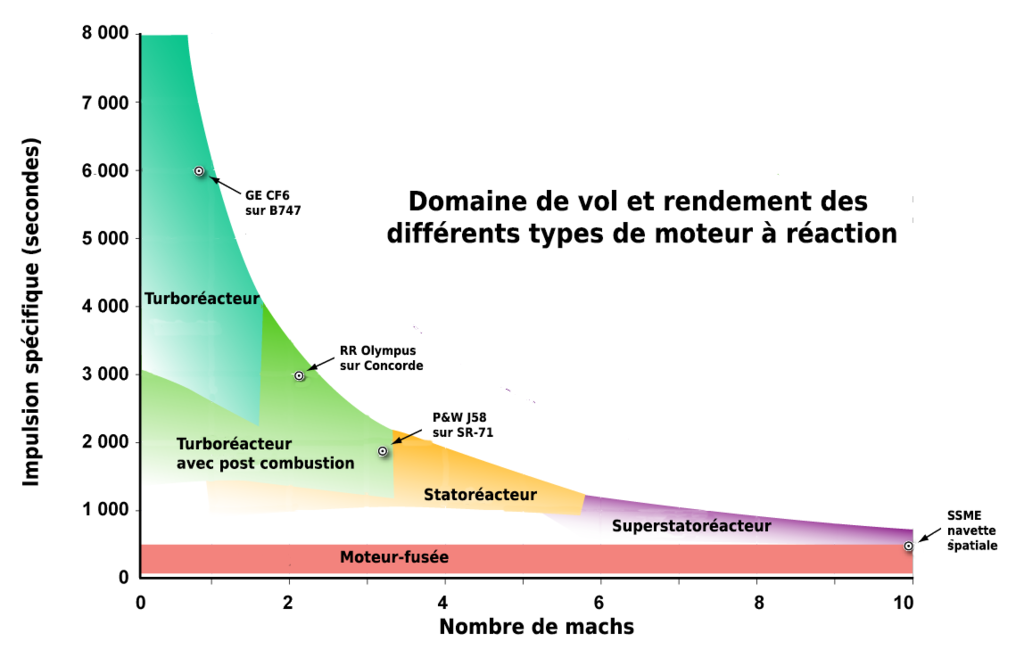
\includegraphics[scale=0.4]{51.JPG}
    \caption{Impulsion spécifique en fonction du nombre de Mach : Quelques valeurs}
    \label{51}
\end{figure}


\section{Déterminer l'équation du $\Delta V$ pour $D=g=0$ et $D=0$, $g = cste$}

L'équation générale d'une fusée est :

\begin{eqnarray}
\boxed{M\dfrac{dV}{dt}=T-D-M_{g_x}}
\end{eqnarray}

\subsubsection{Cas 1 : pas de traînée, pas de gravité (equation de la fusée idéale)}

Equation de Tsiolkovski :

\begin{eqnarray}
\boxed{V-V_0=c ln\left(\dfrac{M_0}{M_{final}}\right)=I_{sp} g_0 ln\left(\dfrac{M_0}{M_{final}}\right)}
\end{eqnarray}

\subsubsection{Cas 2 : Pas de traînée mais gravité}

\begin{eqnarray}
\boxed{V-V_0=c ln\left(\dfrac{M_0}{M_{final}}\right) - \int_{T_0}^{t}g_x dt}
\end{eqnarray}

avec $\int_{T_0}^{t}g_x dt$ la perte due à la gravité qui dépend de la trajectoire.

\section{Comment obtenir un $\Delta V$ supérieur ?}

La vitesse finale peut être obtenue comme :
\begin{eqnarray}
\Delta V_{final} = \Delta V_{in}+\Delta V_{gravite} +\Delta V_{atm}+\Delta V_{???}
\end{eqnarray}

Pour atteindre une vitesse supérieure, on peut 
\begin{itemize}
    \item changer le moteur ($T~\uparrow$) mais le moteur sera plus gros ($\mu \downarrow$)
    \item Avoir une plus grande $I_{sp}$ (différent type de propergol) but $\mu \downarrow$
\end{itemize}



\section{Pourquoi le multi-staging est-il nécessaire (+ expliquer avantages/inconvénients d'étages parallèles ou en série)}

On démontre qu'une fusée composée d'un seul étage ne pourrait placer en orbite une charge utile même si elle utilise les ergols les plus performants et que son indice constructif est particulièrement faible.

Pour optimiser ses performances, une fusée doit donc être multiétages : chaque étage est doté de son ou de ses propres moteurs-fusées et est largué lorsque le carburant est épuisé. Le moteur de l'étage suivant est alors allumé.

\begin{figure}[h!]
    \centering
    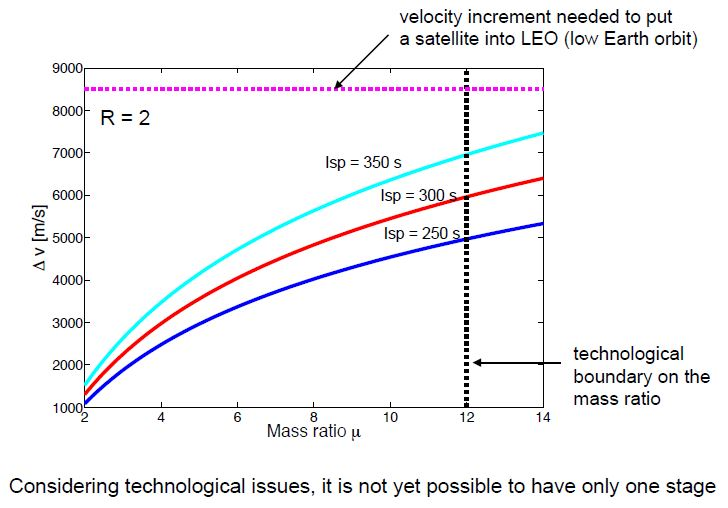
\includegraphics[scale=0.6]{52.JPG}
    \caption{Limite des fusées mono-étagées}
    \label{52}
\end{figure}

\begin{figure}[h!]
    \centering
    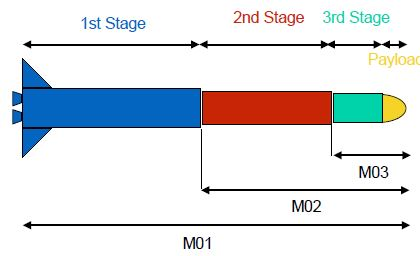
\includegraphics[scale=0.6]{53}
    \caption{Fusée multi-étage}
    \label{53}
\end{figure}

Dans le multi-étage \textbf{en série} (figure \ref{54}), il y a un petit second étage qui est placé au-dessus du premier plus grand. Le premier étage est utilisé au décollage et brûle jusqu'à épuisement de son propergol. Il est ensuite largué et le second étage est allumé. La charge utile est bien évidemment dans l'étage supérieur.

\begin{figure}[h!]
    \centering
    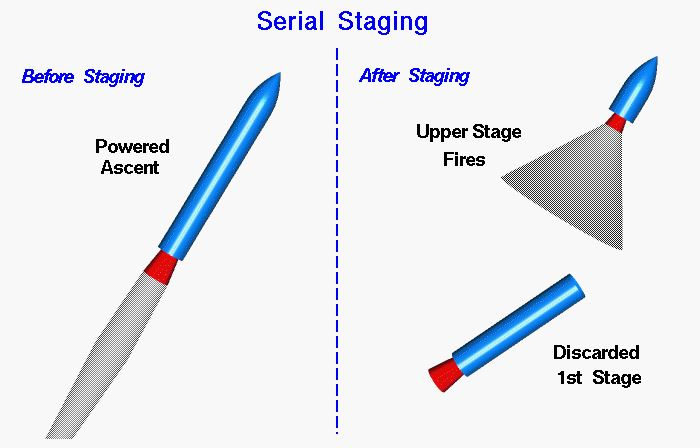
\includegraphics[scale=0.4]{54}
    \caption{Étages en série}
    \label{54}
\end{figure}

Dans le multi-étage \textbf{parallèle} (figure \ref{55}), il y a a de petits étages de chaque côté de l'étage central. Au lancement, tous les étages sont allumés. Lorsque le propergol dans les petits étages est consommé, ils sont largués. L'étage central continue de brûler jusque dans l'espace et contient la charge utile dans sa partie haute.

\begin{figure}[h!]
    \centering
    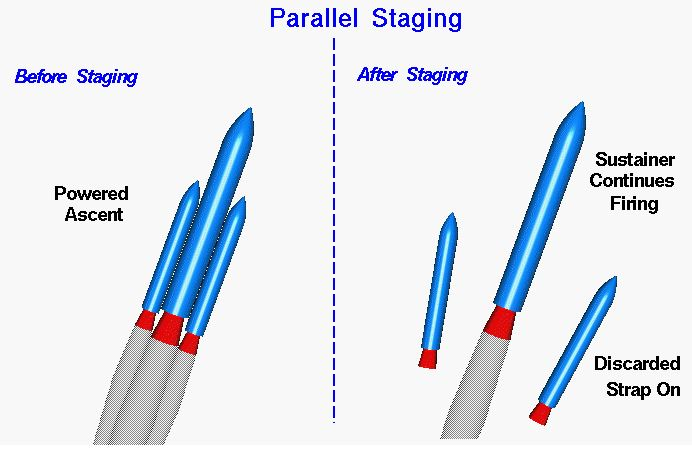
\includegraphics[scale=0.4]{55}
    \caption{Étages parallèles}
    \label{55}
\end{figure}

\subsubsection{Avantages/inconvénients du multi-staging :}

\begin{itemize}
    \item Étagement parallèle :\\
    \textbf{+} : tous les moteurs fonctionnent\\
    \textbf{-} : On ne peut pas optimiser les moteurs pour une partie spécifique de la trajectoire
    \item Étagement en série :\\
    \textbf{+} : On peut optimiser les moteurs pour une partie de la trajectoire\\
    \textbf{-} : Tous les moteurs ne fonctionnent pas (masse en plus)
\end{itemize}

\subsubsection{Optimisation de l'étagement en série :}

Il faut minimiser le rapport de masse final : $\left(\dfrac{M_{01}}{M_{payload}}\right)_min$\\


\begin{eqnarray}
\Delta V_{tot} &= &\Delta V_{orbit}+\Delta V_{gravite} +\Delta V_{atm}\\
g(\mu_1,\mu_2,\mu_3) &= &\sum_{i=1}^N c ln(\mu)-\Delta V_{tot} = 0\\
 M_{oi} &= &M_{oi-1}-M_{prop,i-1}-M_{struct,i-1} \\
\sigma_i &= &\dfrac{M_{struct,i}}{M_{struct,i}-M_{prop,i}}\\
\mu_i &= &\dfrac{M_{o,i}}{M_{o,i}-M_{prop,i}}\\
\dfrac{M_{o,i}}{M_{o,i}-M_{p,i}-M_{s,i}} &= &\dfrac{\mu_i(1-\sigma_i)}{(1-\mu_i\sigma_i}\\
\dfrac{M_{o,i}}{M_{payload}} &= &\Pi_{i=1}^N\dfrac{\mu_i(1-\sigma_i)}{(1-\mu_i\sigma_i)}
\end{eqnarray}

On veut minimiser $\dfrac{M_{o,i}}{M_{payload}}$ par rapport à $\mu_i$. Cela revient à minimiser $ln\left(\dfrac{M_{o,i}}{M_{payload}}\right)$
\begin{eqnarray}
ln\left(\dfrac{M_{o,i}}{M_{payload}}\right) &= &\sum_{i=1}^N \left(ln(\mu_i)+ln(1-\sigma_i)-ln(1-\sigma_i\mu_i)\right)\\
F &= &\sum_{i=1}^N \left(ln(\mu_i)+ln(1-\sigma_i)-ln(1-\sigma_i\mu_i)\right) + \lambda\sum_{i=1}^N c_iln(\mu_i)-\Delta V_{tot}
\end{eqnarray}

avec $\lambda\sum_{i=1}^N c_iln(\mu_i)-\Delta V_{tot}$ les contraintes.

\[
\begin{cases}
\dfrac{\partial F}{\partial\mu_i} = \dfrac{1}{\mu_i}\left(\dfrac{-\sigma_i}{1-\mu_i\sigma_i}\right) + \lambda c_i\dfrac{1}{\mu_i}=0\\
\dfrac{\partial F}{\partial\lambda}=\sum_{i=1}{N}c_i ln(\mu_i)-\Delta V_{tot} = 0
\end{cases}
\]



\section{Quels sont les objectifs et phases de la trajectoire de vol}

Objectifs :
\begin{itemize}
    \item Minimiser les contraintes sur le lanceur $\dfrac{\rho V^2 S}{2}$
    \item Minimiser les pertes dues à la gravité
\end{itemize}

Il y a deux phases lors d'un vol :
\begin{itemize}
    \item \textit{La phase verticale} : peu de contraintes mais beaucoup de pertes gravitationnelles
    \item \textit{La trajectoire inclinée} : plus de contraines structurales mais moins de pertes gravitationnelles
\end{itemize}


\section{Expliquer les trois types de rendez-vous }

\subsubsection{Cas 1 : Orbite de l'intercepteur (orbite en phase) $\ne$ orbite cible }

\begin{figure}[h!]
    \centering
    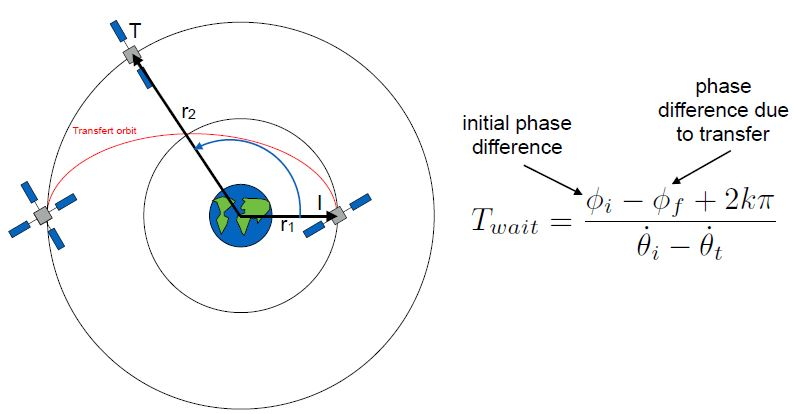
\includegraphics[scale=0.6]{57.JPG}
    \caption{Rendez-vous 1}
    \label{57}
\end{figure}

\subsubsection{Cas 2 : Intercepteur et cible sur le même orbite. Ils ont besoin d'être en phases différentes }

\begin{figure}[h!]
    \centering
    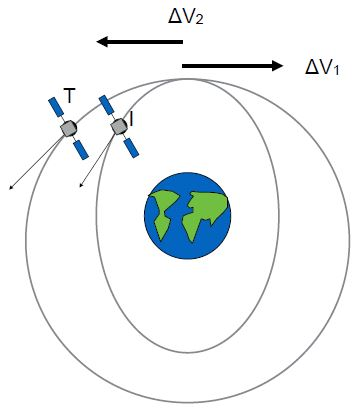
\includegraphics[scale=0.6]{58.JPG}
    \caption{Rendez-vous 2}
    \label{58}
\end{figure}

\subsubsection{Cas 3 : Intercepteur et cible}

\begin{figure}[h!]
    \centering
    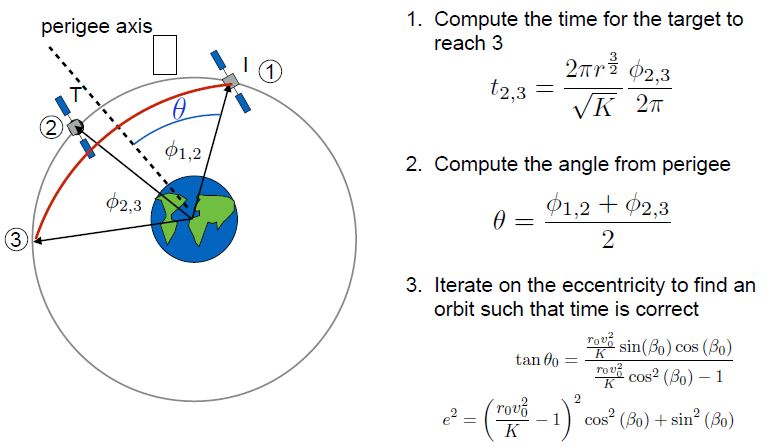
\includegraphics[scale=0.6]{59.JPG}
    \caption{Rendez-vous 3}
    \label{59}
\end{figure}




\section{Expliquer les transferts interplanétaires + l'assistance gravitationnelle}

\begin{figure}[h!]
    \centering
    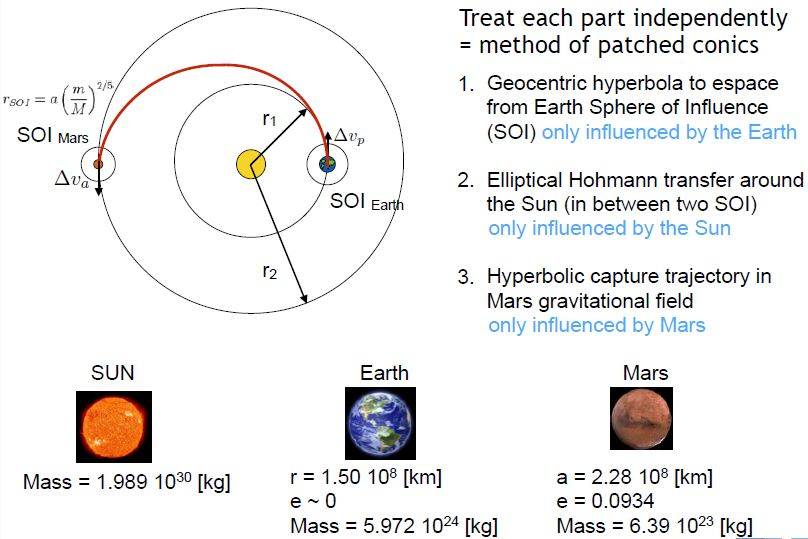
\includegraphics[scale=0.6]{60.JPG}
    \caption{Transfert interplanétaire}
    \label{60}
\end{figure}

\textbf{Assistance gravitationnelle} : utiliser l'attraction d'autre corps célestes (lunes, planètes,...) pour réaliser tes variations de trajectoire et de vitesse.



\end{document}
